\documentclass[10pt]{article}

\usepackage[margin=1in]{geometry}
\usepackage{amsmath}
\usepackage{amssymb}
\usepackage{amsthm}
\usepackage{mathtools}
\usepackage{bm}

\usepackage{color}
\usepackage{colortbl}
\definecolor{deepblue}{rgb}{0,0,0.5}
\definecolor{deepred}{rgb}{0.6,0,0}
\definecolor{deepgreen}{rgb}{0,0.5,0}
\definecolor{gray}{rgb}{0.7,0.7,0.7}

\usepackage{hyperref}
\hypersetup{
  colorlinks   = true, %Colours links instead of ugly boxes
  urlcolor     = black, %Colour for external hyperlinks
  linkcolor    = blue, %Colour of internal links
  citecolor    = blue  %Colour of citations
}

%%%%%%%%%%%%%%%%%%%%%%%%%%%%%%%%%%%%%%%%%%%%%%%%%%%%%%%%%%%%%%%%%%%%%%%%%%%%%%%%

\theoremstyle{definition}
\newtheorem{problem}{Problem}
\newtheorem{defn}{Definition}
\newcommand{\R}{\mathbb R}
\DeclareMathOperator{\vcdim}{VCdim}
\DeclareMathOperator{\E}{\mathbb E}
\DeclareMathOperator{\nnz}{nnz}
\DeclareMathOperator{\determinant}{det}
\DeclareMathOperator{\Var}{Var}
\DeclareMathOperator{\rank}{rank}
\DeclareMathOperator*{\argmin}{arg\,min}
\DeclareMathOperator*{\argmax}{arg\,max}

\newcommand{\I}{\mathbf I}
\newcommand{\Q}{\mathbf Q}
\newcommand{\p}{\mathbf P}
\newcommand{\pb}{\bar {\p}}
\newcommand{\pbb}{\bar {\pb}}
\newcommand{\pr}{\bm \pi}
\newcommand{\epsapp}{\epsilon_{\text{app}}}
\newcommand{\epsest}{\epsilon_{\text{est}}}

\newcommand{\trans}[1]{{#1}^{T}}
\newcommand{\loss}{\ell}
\newcommand{\w}{\mathbf w}
\newcommand{\x}{\mathbf x}
\newcommand{\y}{\mathbf y}
\newcommand{\lone}[1]{{\lVert {#1} \rVert}_1}
\newcommand{\ltwo}[1]{{\lVert {#1} \rVert}_2}
\newcommand{\lp}[1]{{\lVert {#1} \rVert}_p}
\newcommand{\linf}[1]{{\lVert {#1} \rVert}_\infty}
\newcommand{\lF}[1]{{\lVert {#1} \rVert}_F}

\newcommand{\h}{\mathcal H}
\newcommand{\D}{\mathcal D}
\DeclareMathOperator*{\erm}{ERM}

%%%%%%%%%%%%%%%%%%%%%%%%%%%%%%%%%%%%%%%%%%%%%%%%%%%%%%%%%%%%%%%%%%%%%%%%%%%%%%%%

\begin{document}


\begin{center}
\Huge
Notes: Model Zoo
\end{center}

\begin{center}
    \hspace*{-0.75in}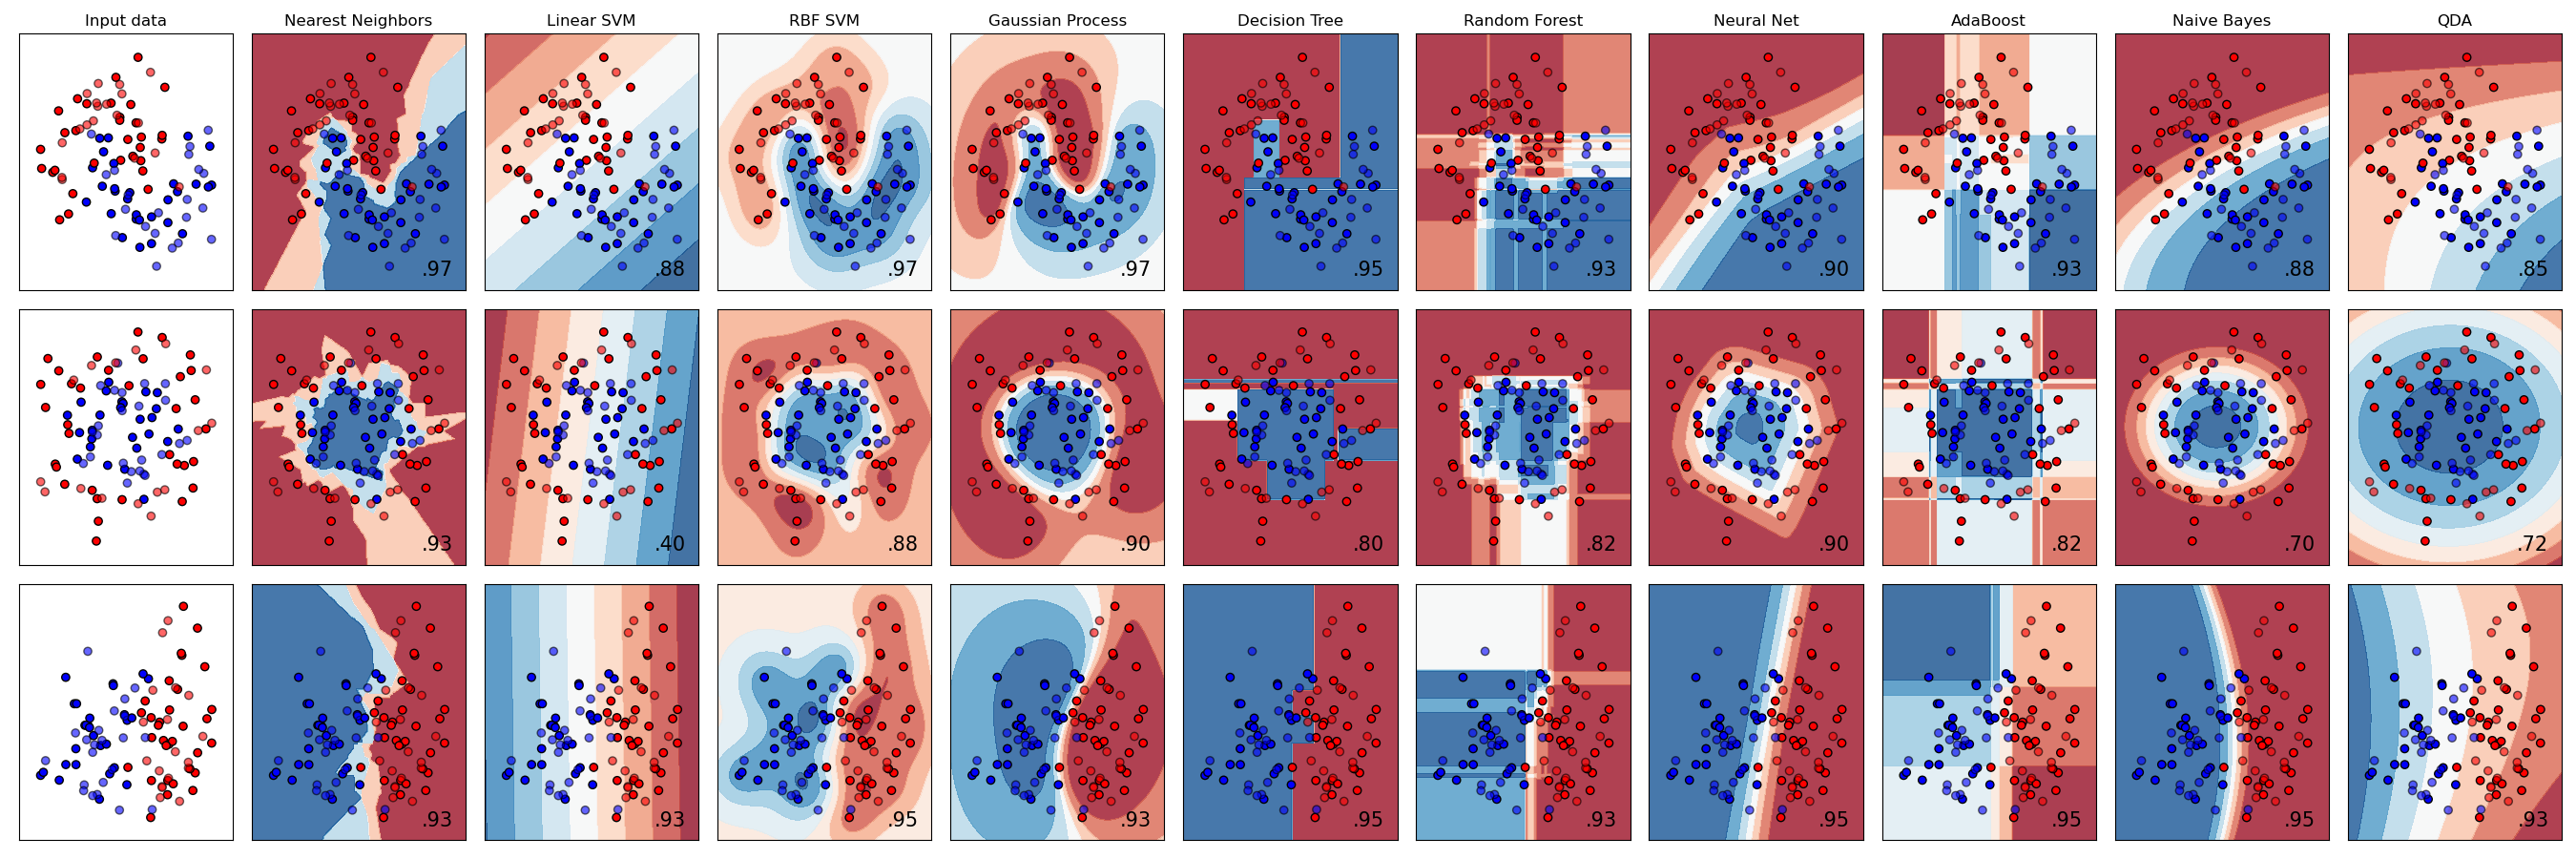
\includegraphics[width=8in]{sphx_glr_plot_classifier_comparison_001}
    \small
    Source: \url{https://scikit-learn.org/stable/auto_examples/classification/plot_classifier_comparison.html}
\end{center}

%%%%%%%%%%%%%%%%%%%%%%%%%%%%%%%%%%%%%%%%%%%%%%%%%%%%%%%%%%%%%%%%%%%%%%%%%%%%%%%%

\section{Pre-lecture Work}

None.
Get plenty of sleep and do well on all your midterms :)

%\begin{problem}
    %\begin{enumerate}
        %\item Theorem 11.1
        %\item Theorem 11.2
        %\item Draw the model selection curve
    %\end{enumerate}
%\end{problem}

%%%%%%%%%%%%%%%%%%%%%%%%%%%%%%%%%%%%%%%%%%%%%%%%%%%%%%%%%%%%%%%%%%%%%%%%%%%%%%%%

\section{Lecture}

\begin{problem}
    What is a decision boundary?
\end{problem}

\newpage
\begin{problem}
    What is a universal approximation theorem?
\end{problem}

\newpage
\begin{problem}
    Neural Networks.
    \begin{enumerate}
        \item Optional Videos:
            \begin{enumerate}
                \item 3Blue1Brown on Neural Networks: \url{https://www.youtube.com/watch?v=aircAruvnKk&list=PLZHQObOWTQDNU6R1_67000Dx_ZCJB-3pi}
            \end{enumerate}
        \item What is the hypothesis class of 1-layer neural networks?
            \vspace{3in}
        \item What is the hypothesis class of n-layer neural networks?
            \vspace{3in}
        \item What is the VC-dimension of neural networks? (Theorem 20.6)
            \vspace{3in}
        %\item 
            %Modern ``deep learning'' systems have many layers that are very wide.
    \end{enumerate}
\end{problem}

\newpage
\begin{problem}
    Decision Trees
    \begin{enumerate}
        \item Optional Videos:
            \begin{enumerate}
                \item StatQuest on decision trees: \url{https://www.youtube.com/watch?v=7VeUPuFGJHk}
                \item StatQuest on regression trees: \url{https://www.youtube.com/watch?v=g9c66TUylZ4}
            \end{enumerate}
        \item What is the hypothesis class of decision stumps?
            \vspace{3in}
        \item What is the hypothesis class of depth $k$ decision trees?
            \vspace{3in}
        \item What is the VC-dimension of depth $k$ decision trees?
            \vspace{3in}
    \end{enumerate}
\end{problem}

\newpage
\begin{problem}
    Ensemble Methods
    \begin{enumerate}
        \item Optional Videos:
            \begin{enumerate}
                \item StatQuest on random forests: \url{https://www.youtube.com/watch?v=J4Wdy0Wc_xQ}
                \item StatQuest on AdaBoost: \url{https://www.youtube.com/watch?v=LsK-xG1cLYA}
                \item StatQuest on XGBoost (4 videos): \url{https://www.youtube.com/watch?v=OtD8wVaFm6E&list=PLblh5JKOoLUICTaGLRoHQDuF_7q2GfuJF&index=57}
                \item Alex Ihler on bagging: \url{https://www.youtube.com/watch?v=Rm6s6gmLTdg}
            \end{enumerate}
        \item What is the hypothesis class of ensemble methods?
            \vspace{3in}
        \item What is the VC-dimension of ensemble methods?
            \vspace{3in}
    \end{enumerate}
\end{problem}

\newpage
\begin{problem}
    Nearest Neighbor
    \begin{enumerate}
        \item Optional Videos:
            \begin{enumerate}
                \item StatQuest: \url{https://www.youtube.com/watch?v=HVXime0nQeI}
            \end{enumerate}
        \item What is the $k$-nearest neighbor classification rule?
            \vspace{3in}
        \item What is the VC-dimension of $k$-nearest neighbor?
            \vspace{3in}
        \item Nearest neighbor can still be effective in practice.  Why?
    \end{enumerate}
\end{problem}

%\newpage
%\begin{problem}
    %Humans
    %\begin{enumerate}
        %\item What is the hypothesis class of 
    %\end{enumerate}
%\end{problem}

\end{document}


